\gls{wrtc} deviates from traditional enterprise communications in two ways: it opens up communications from every web application instead of controlled software pieces. The integration of \gls{wrtc} with legacy systems could happen in the end user's browser (client) or via a translation gateway (server).

In this chapter we will explore the technical requirements for integrating RTCWEB with a typical enterprise communications system architecture and give the suggested solution about the requirements. Then analyse some of the problems raised by the integration.

Translation of bothe singaling and media is necessary.

\section{Interoperation}
There are two ways of going about this problem. We can either choose to redo the whole existing architecture of the enterprise communication system putting WebRTC technology in the center and upgrade all the existing infrastructure to support WebRTC, but this is an expensive solution, especially since the IETF has not yet finished deciding upon which protocols and codec to be used. Therefore, the best option is to extend current architecture with WebRTC capabilities. To do this we have to create a gateway between the underlying technologies of WebRTC specified as RTCWeb and existing enterprise infrastructure. The aim when creating a gateway between the two systems is to re-use as much as possible of existing architecture.

\subsection{Requirements and problems}
There are basically three planes we have to make interoperate: the signaling plane, the media plane, and the IP addressing plane. 
By signaling we mean the offer/answer exchange. The media plane is the transportation of the media, and the IP addressing plane is basically how we connect to each other.

\begin{figure}[here]
\centerline{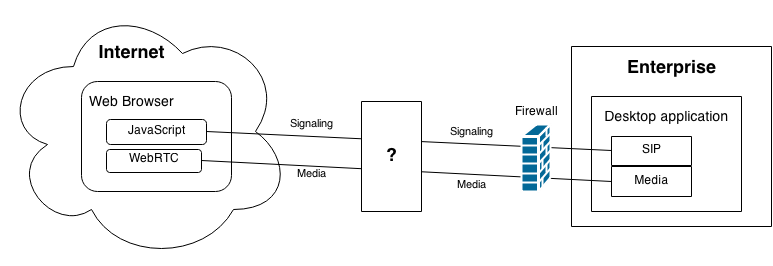
\includegraphics[scale=0.5]{gateway-layers.png}}
\caption{WebRTC-Enterprise interworking}
\label{fig:gateway-layers}
\end{figure}

\subsubsection{Signaling}
WebRTC does not define any standard way of doing signaling, but we do have to implement it and get it working with typical enterprise ways of doing this. In order to get a session going, the peers basically need to exchange four things\cite{??}:

\begin{itemize}
\item{An ICE username}
\item{An ICE password}
\item{A list of possible ICE candidates}
\item{A DTLS fingerprint}
\end{itemize}

The current WebRTC specification says to exchange this information with the browser API in SDP format. SDP is an old format used in the VoIP world, therefore the re-use of SDP is supposed to save time, but the anatomy of an SDP is complex and constantly changing because the IETF are coming up with new stuff to include. All the information has to be excactly right or it will be rejected by the browser. It is highly unlikely that the current specification of SDP will work with any older implementation found in any enterprise communication system.

Another thing is that WebRTC has to do signaling running over HTTP, while the standard in an enterprise system is to use SDP with SIP or some other proprietary way over TCP or UDP.

We need to come up with some way of manipulating the SDP and possibly use a SIP stack developed in Javascript running in the client.

\subsubsection{Media}
In the \gls{wrtc} world the media plain is designed to avoid having to relay media streams. The goal is to have pure peer-to-peer connections, while in the enterprise world it is common to have full control over the media plane and in most cases use some kind of media server. Also the WebRTC specification says that support for ICE and SRTP-DTLS are mandatory. Encryption is hardly ever used in the enterprise world, so this is another challenge. If encryption is used, it is more common to use SRTP-SDES with the keys being handled on the signaling plane, rather than in media plane that is the case with DTLS.

WebRTC uses one-way media streams, while an enterprise system usually expects to receive bi-directional streams. This can be fixed by multiplexing the streams, so we can have multiple streams running over the same network port.

The biggest issues here is probably which codecs we need to implement. The IETF has landed on two default audio codecs, but has not decided on which video codec to use yet. The most typical enterprise video code used is H.264. Right now the IETF are deciding between VP8 and H.264, so currently we have to support both and do server side transcoding between them.

\subsubsection{IP addressing}
In the enterprise world a SBC is commonly used to control incoming media traffic. In WebRTC one uses ICE browser-to-browser to cross NATs/Firewalls. We have to handle both exchanging of ICE candidates and bypassing the enterprise firewall. This is a bigger topic that we will go more deeply into in the next chapter.

\subsection{Integration}
Simple way:
Using SIP-over-WebSocket signaling and use an end-to-end media path enabled by \gls{wrtc}. This could work if the legacy enterprise system supported all the required protocols defined in \gls{wrtc}, otherwise the architecture would have to be upgraded to support all the new features. This is not trivial, since it would require to redo all of the existing architecture just to support \gls{wrtc}. It is better to create a bridge in the form of a gateway between \gls{wrtc} and the legacy architecture.

The gateway:

First showing a simple web application P2P WebRTC structure. Here signaling goes through a signaling server and media travels directly between the two peers(browsers).

\begin{figure}[here]
\centerline{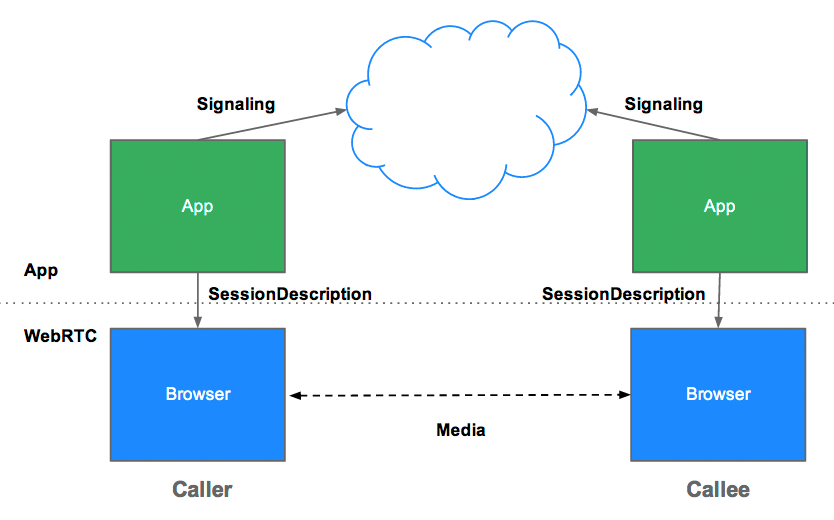
\includegraphics[scale=0.3]{jsep.png}}
\caption{WebRTC P2P architecture}
\label{fig:jsep}
\end{figure}

Secondly showing a typical enterprise architecture with signaling server, media server, and a server for routing the streams to peers.

\begin{figure}[here]
\centerline{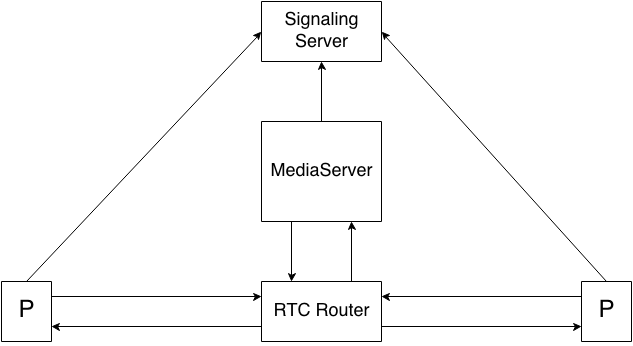
\includegraphics[scale=0.3]{VirtualArena.png}}
\caption{Enterprise communication platform architecture}
\label{fig:VirtualArenaArchitecture}
\end{figure}

Let's see how RTCWeb can be used to connect to existing enterprise communication networks.

In the solution figure we add an interworking gateway component. This component includes three subcomponents(signaling gateway, media relay gateway, and address server(address translation)). These provide all the necessary functionality.

%figure


\subsection{Summary}
The first iteration of RTCWeb is still under development, and not all protocols and codecs have been decided yet. It is theoretically possible to create a gateway and it has been done before under closed doors. Some of the biggest issues are how to handle the signaling, translating the media, and crossing the enterprise firewall.


% \subsection{Related Work}
% There is a great interest in interworking webRTC with existing telco services. An example is the integration with IMS. This work closely resembles the work that is done in this thesis. Currently there are gateway implemenations between webrtc and ims created by ericsson and mavenir. the 3gpp is doing work on drafting a standardized gateway implementation between webrtc and ims. Both ericsson and mavenir systems are closed to th epublic, but the 3gpp papers are open for reviewing.